\documentclass{article}
\usepackage{tikz,lipsum,lmodern}
\usepackage{epsfig,graphicx,subfigure,amsthm,amsmath}
\usepackage{fontspec}
\usepackage{color,xcolor} 
\usepackage{xepersian}
\settextfont[Scale=1]{BZAR.TTF}
\usepackage[inline]{asymptote}
\newcommand{\half}{\frac12}
\usepackage{amsmath} 
\usepackage{xcolor}
\usepackage{hyperref}
\usepackage[breakable,most]{tcolorbox}
\renewcommand{\headrulewidth}{.4mm} % header line width 
\usepackage{fancyhdr}

\pagestyle{fancy}
\fancyhf{}
\fancyhfoffset[L]{1cm} % left extra length
\fancyhfoffset[R]{1cm} % right extra length
\rhead{\today}
\lhead{\bfseries قضیه کیسی و کاربرد ها}
\rfoot{صفحه~\thepage}


\hypersetup{ 
colorlinks=true,
linkcolor=blue,
filecolor=blue,
citecolor = black,
urlcolor=magenta,
}

\author{ایمان قادر \and  مهران طلایی }
\title{قضیه کیسی و کاربرد ها}

\begin{document}
\maketitle

\begin{abstract}
قضیه کیسی از قضایای کلاسیک و پر استفاده در هندسه است که با توجه به کمبود متریال آموزشی در حیطه این مبحث ولی کاربرد زیاد آن، به گرد آوری این مقاله روی آوردیم که شامل تعاریف و قضایای مورد نیاز و همینطوری از هر بخش مثال هایی مطرح شده اند که به یادگیری هرچه بیشتر کمک میکنند. و در انتها تمرین هایی برای دست ورزی و خودآزمایی قرار داده شده است.
\end{abstract}

\newtcbtheorem[breakable,enhanced ,pad at break*=1mm,auto counter,number within=section]{theo}%
  {قضیه}{
     arc=0mm, colback=blue!5!white,colframe=blue!75!black}{theorem}
  
  
\newtcbtheorem[enhanced jigsaw,breakable,pad at break*=1mm,auto counter,number within=section]{exam}%
  {مثال}{
     arc=0mm, colback=green!5!white,colframe=green!30!black}{example}
\newtcbtheorem[enhanced jigsaw,breakable,pad at break*=1mm]{defi}%
  {تعریف }{
     arc=0mm, colback=black!5!white,colframe=white!30!black}{definition}
     
ابتدا با یک تعریف شروع میکنیم:
\begin{defi}{}{}
تابع اختلاف قوت نقطه $P$ نسبت به دو دایره $\omega_1$ و $\omega_2$ را به شکل زیر تعریف میکنیم:
\[\mathbf{P}(P,\omega_1,\omega_2)=Pow_{\omega_1}^P -Pow_{\omega_2}^P\]
\end{defi}

\section{صورت قضیه کیسی}

\begin{theo}{}{}
فرض کنید که دوایر $\omega_1$ و $\omega_2$ به مراکز $O_1$ و $O_2$ در صفحه هستند و خط $l$ محور اصلی این دو دایره است و نقطه $P$ نقطه ای در صفحه $\omega_1$ و $\omega_2$ است. آنوقت رابطه زیر برقرار است:
\[\mathbf{P}(P,\omega_1,\omega_2)=2dist(P,l) \overline{O_1O_2} \]
\end{theo}
\bold{اثبات:}

\begin{center}
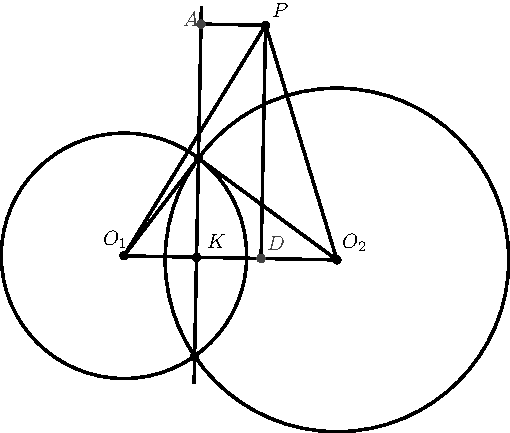
\includegraphics[scale=0.6]{caseypro.pdf}
\end{center}
دوایر $\omega_1(O_1,r_1)$ و  $\omega_2(O_2,r_2)$ را در نظر بگیرید. و $A$ و $D$  به ترتیب پاهای عمود از $P$ بر محور اصلی و خط المرکزین این دو دایره هستند. حال داریم:
\begin{align*}
Pow_{\omega_1}^P-Pow_{\omega_2}^P &= PO_1^2-r_1^2-PO_2^2+r_2^2 \\
&= DO_1^2-DO_2^2+r_2^2-r_1^2 \\
&=(DO_1-DO_2)\overline{O_1O_2}+KO_1^2-KO_2^2\\
&=(DO_1-DO_2)\overline{O_1O_2}+(KO_1-KO_2)\overline{O_1O_2} \\
&=(DO_1-DO_2+KO_1-KO_2)\overline{O_1O_2}\\
&=2 \overline{PA} \thickspace\overline{O_1O_2} \thickspace \blacksquare
\end{align*}



\begin{exam}{}{}
دایره $\omega'$ دایره ای به مرکز $O'$  به طور کامل درون دایره $\omega$ و مرکز $O$ قرار دارد. نقاط $A$ و $B$ به گونه ای بر روی دایره $\omega$ قرار دارند که  $\overline{AB}$ بر $\omega'$ مماس است. دایره $\Omega$  را دایره محیطی $\triangle{O'AB}$ در نظر بگیرید. خط $\overline{AB}$ را با حفظ جهت حرکت میدهیم مکان هندسی مرکز $\Omega$ را بیابید.
\end{exam}
\bold{اثبات:} مرکز $\Omega$ را $O''$ مینامیم.

\begin{center}
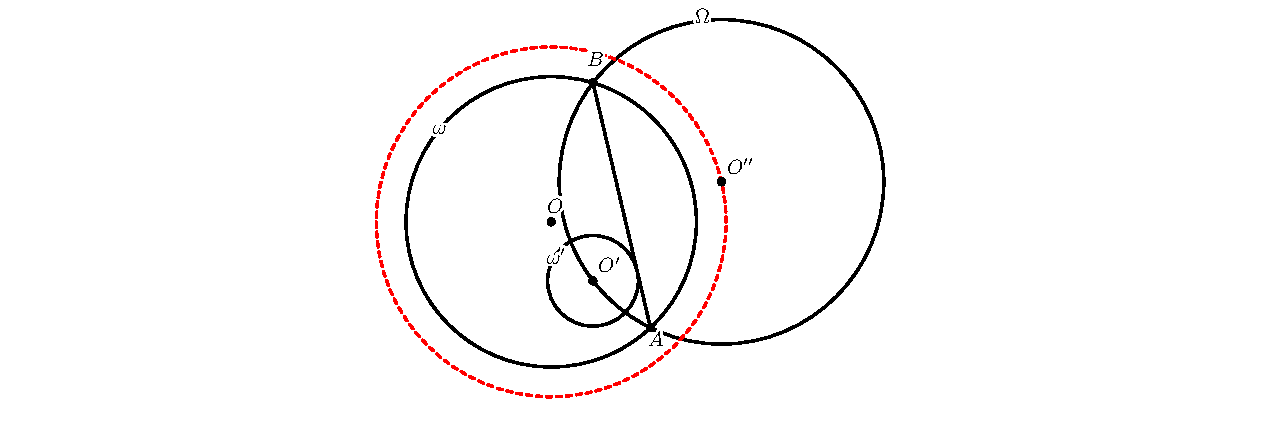
\includegraphics[scale=0.6]{ncavenye.pdf}
\end{center}

حال $\mathbf{P}(O',\omega,\Omega)$ را محاسبه میکنیم:
\begin{align*}
\mathbf{P}(O',\omega,\Omega)=Pow_{\omega}^{O'}-Pow_{\Omega}^{O'}&=2 R_{\omega'} \overline{OO''}\\
\leftrightarrow \frac{Pow_{\omega}^{O'}-0}{2 R_{\omega'}}&=\overline{OO''}
\end{align*}
بنابر این طول $OO''$ ثابت است و این نتیجه میدهد که مکان هندسی $O''$ دایره ای است به مرکز $O$ و شعاع $\frac{Pow_{\omega}^{O'}}{2 R_{\omega'}}$ .
\begin{exam}{}{}
 $\omega_B$ و $\omega_C$ دوایر محاطی خارجی مثلث $\triangle{ABC}$ هستند. دایره $\omega_B'$ با دایره $\omega_B$ نسبت به وسط $AC$ متقارن هستند و دایره $\omega_C'$ با دایره $\omega_C$ نسبت به وسط $AB$ متقارن هستند. اثبات کنید که محور اصلی  $\omega_B'$ و  $\omega_C'$ محیط مثلث را نصف میکن.  
({روسیه 2005})
\end{exam}
 \bb{اثبات:}    دایره محاطی مثلث را $\omega$ بنامید و محل تماس $\omega_A$ با خط $BC$ را $D$ در نظر میگیریم حال اثبات میکنیم که خط $AD$ محور اصلی دو دایره $\omega_B'$ و $\omega_C'$ است.
\begin{center}
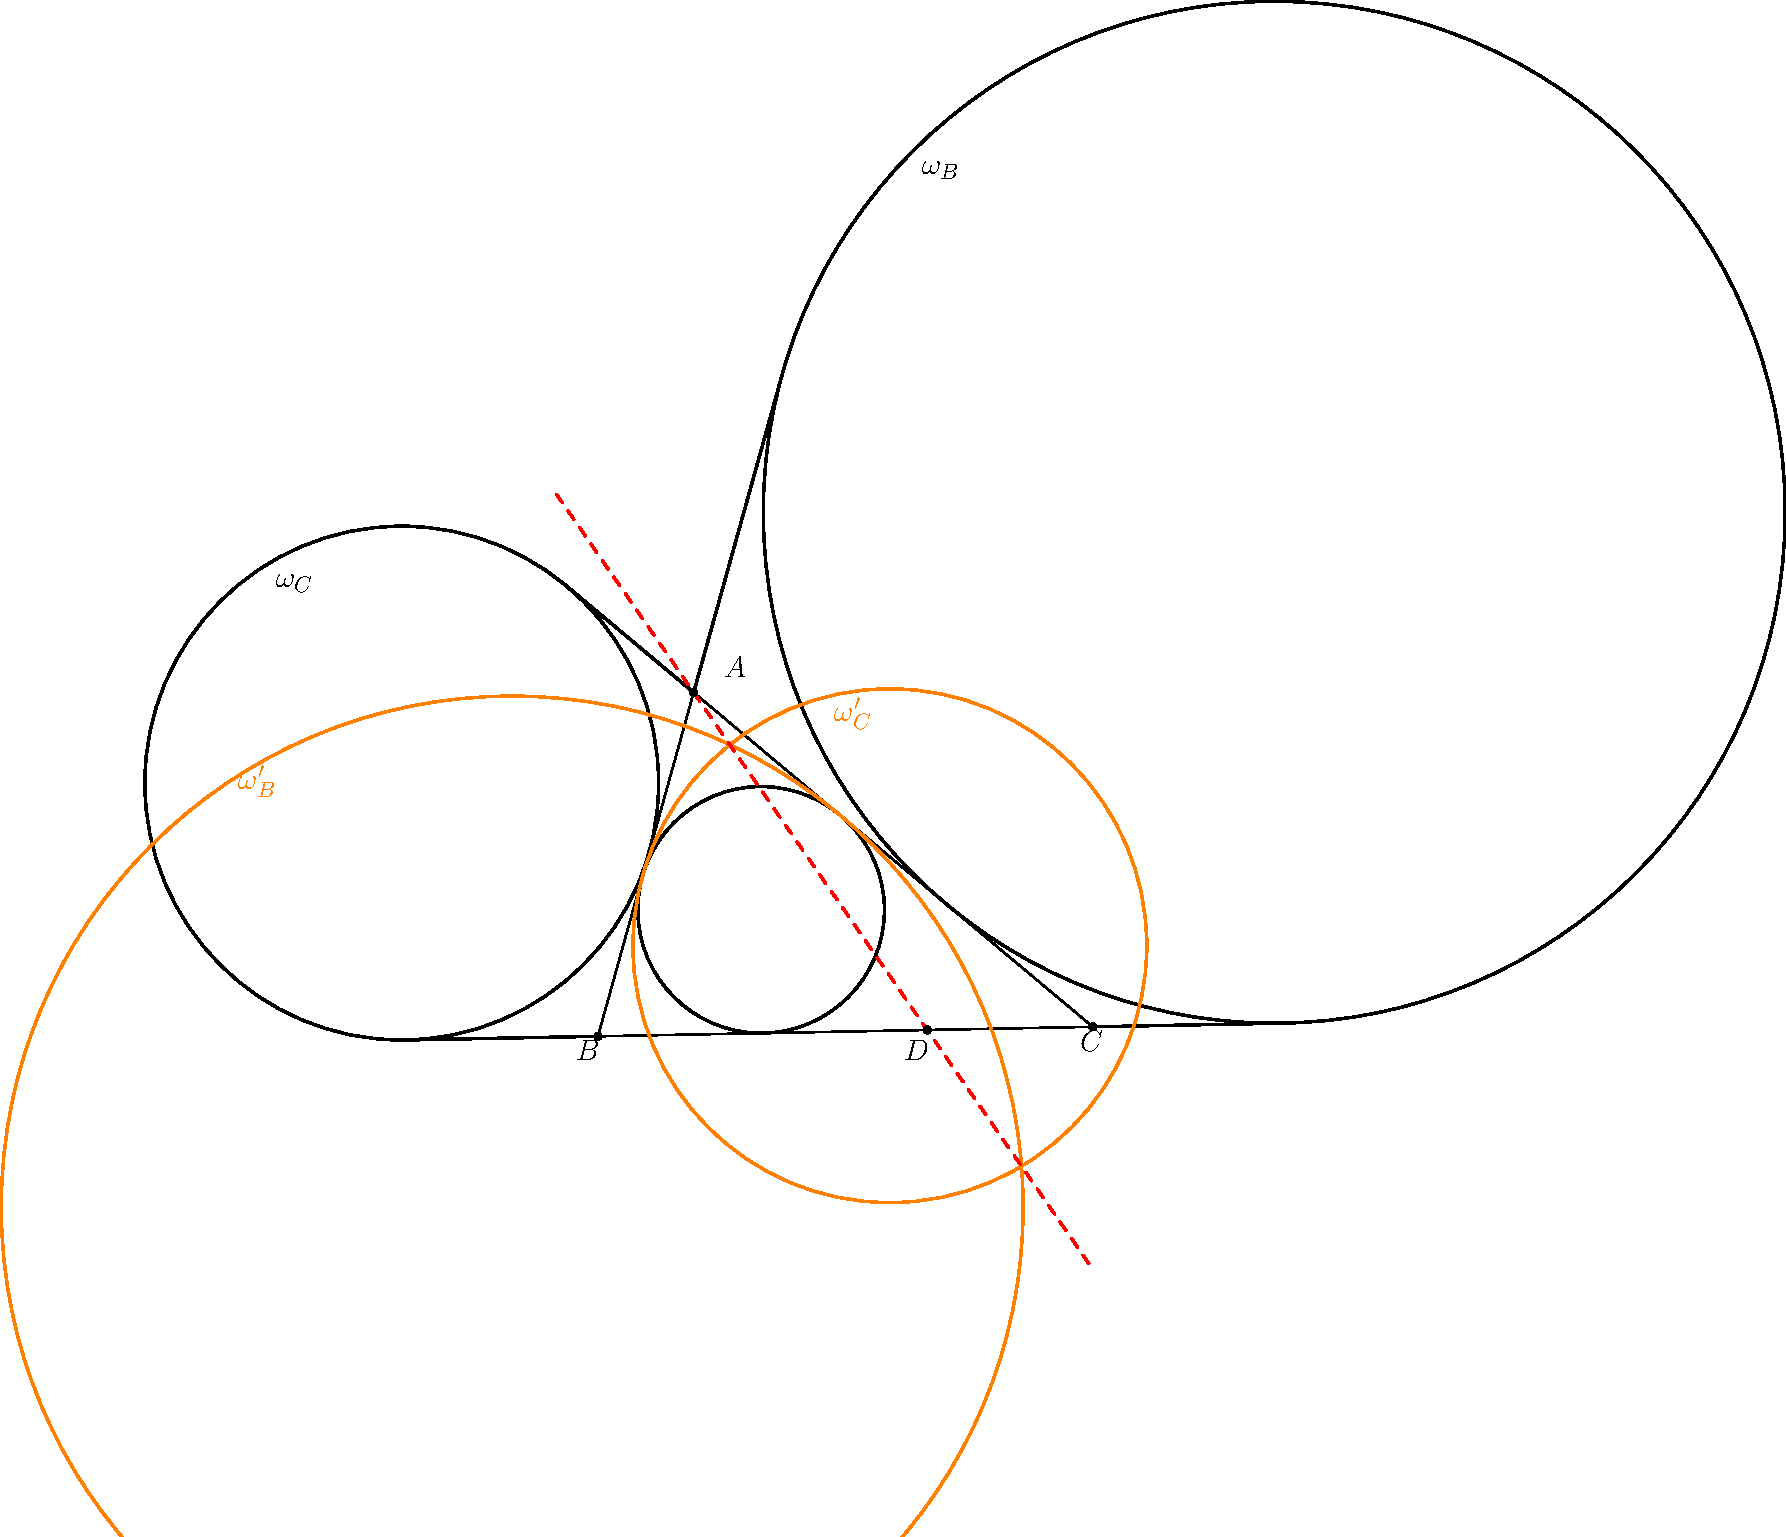
\includegraphics[scale=0.3]{alrussian.pdf}
\end{center}
کافی است بگوییم که:
\[Pow_{\omega}^D-Pow_{\omega_B}^D=Pow_{\omega}^D-Pow_{\omega_C}^D\]
داریم:
\begin{align*}
Pow_{\omega}^D-Pow_{\omega_B}^D&=2 dist(D,\overline{AC}) (r_B-r) \\
&= 2 (p-b) Sin(\angle{ACB}) (r_B-r)
\end{align*}
به نحو مشابه داریم:
\[Pow_{\omega}^D-Pow_{\omega_C}^D=2 (p-c) Sin(\angle{ABC}) (r_C-r)\]
و در نهایت

\begin{align*}
2 (p-c) Sin(\angle{ABC}) (r_C-r)&=2 (p-b)Sin(\angle{ACB}) (r_B-r)\\
\longleftrightarrow
\end{align*}

\section{اختلاف قوت}
\begin{theo}{}{}

‏فرض‎ کنید که دوایر ‎‎$‎\omega_1‎$‎ ‏و ‎‎$‎\omega_2‎$‎ و نقاط همخط ‎‎$‎A‎$ ‎‏‏‏،‎‎$‎B‎$ و ‎$‎‎‎‎‏‎C‎$‎‎‎‎ ‏در یک صفحه هستند. و ‎‎$‎C=\alpha ‎A+(1-\alpha)B‎$‎‎ ‏آنوقت داریم:
‎‎\[‎‎\mathbf{P}(C,\omega_1,\omega_2)=\alpha ‎‎\mathbf{P}(A,\omega_1,\omega_2)+(1-\alpha)‎‎\mathbf{P}(B,\omega_1,\omega_2)‎‎\]
\end{theo}

‎\bold{:‎‏اثبات}

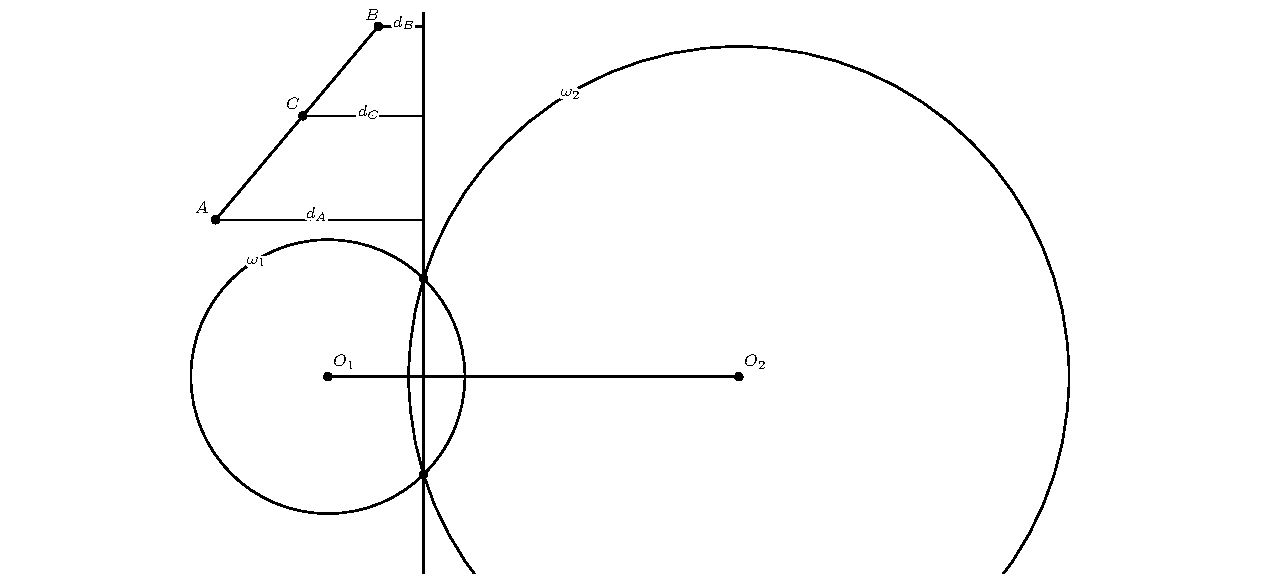
\includegraphics[scale=0.6]{dif.pdf}

فرض کنید که ‎$d_P‎$‎‎ ‏فاصله نقطه ‎$‎P‎$‎‎‎‎ ‏تا محور اصلی ‎‎$‎\omega_1‎$‎ ‏‎‎‏و ‎‎$‎\omega_2‎$‎ ‏باشد. ‎
‏حالا‎‎‎ از قضیه ‎\bold{کیسی}‎ ‏داریم:
\begin{align*}‎‎
\mathbf{P}(C,\omega_1,\omega_2)=2d_cO_1O_2&=\frac{BC}{AB} ‎\times ‎\overbrace{2 d_A O_1O_2}^{‎‎\mathbf{P}(A,\omega_1,\omega_2)}‎+‎‎\frac{AC}{AB} ‎\times ‎\overbrace{2 d_B O_1O_2}^{‎‎\mathbf{P}(B,\omega_1,\omega_2)}‎\\‎
&= ‎\alpha‎ ‎‎\mathbf{P}(A,\omega_1,\omega_2)+(1-\alpha) ‎‎\mathbf{P}(B,\omega_1,\omega_2)
\end{align*}
که به این ترتیب حکم اثبات میشود.\blacksquare

\begin{exam}{}{}
چهاضلعی ‎‎$‎APBQ‎$‎ ‏در دایره ‎‎$‎\omega‎$‎ ‏محاط شده است ‎‎‏به طوری که ‎‎$‎\angle P=\angle ‎Q‎=90^\circ$‎‎‎‎ ‏و\\ ‎‎$‎AP=AQ<BP‎$‏. ‎فرض‎ کنید که ‎‎$‎X‎$‎‎‎‎ ‏نقطه ای متغیر بر روی ‎‎‏پاره خط ‎‎$‎‎\overline{PQ}‎‎$‎ ‏باشد. خط ‎‎$‎AX‎‎‏$‏،‎‎‎‎‎ دایره ‎‎$‎‎\omega‎‎$‎ ‏را برای بار دیگر در نقطه ‎‎$‎S‎$‎ ‏قطع میکند. نقطه ‎$‎‎‎T‎$‎‎‏ ‏به‎‎ روی کمان ‎‎‎$‎AQB‎$‎‎‎‎ ‏از ‎‎$‎‎\omega‎‎$‎ ‏قرار دارد به طوری که ‎‎$‎\overline{XT}‎$‎ ‏بر ‎‎$‎\overline{AX}‎$‎ ‏عمود است. اثبات کنید که اگر ‎‎$‎M‎$‎ ‏را وسط ‎‎$‎\overline{ST}‎$‎‎‎ ‏بنامیم‏، با حرکت ‎‎$‎X‎$‎ ‏روی ‎‏پاره خط ‎$\overline{PQ}‎$‎‎‎‎ ‏مکان هندسی ‎‎$‎M‎$‎ ‏یک دایره است‎.‎
\end{exam}
\newpage
اثبات:

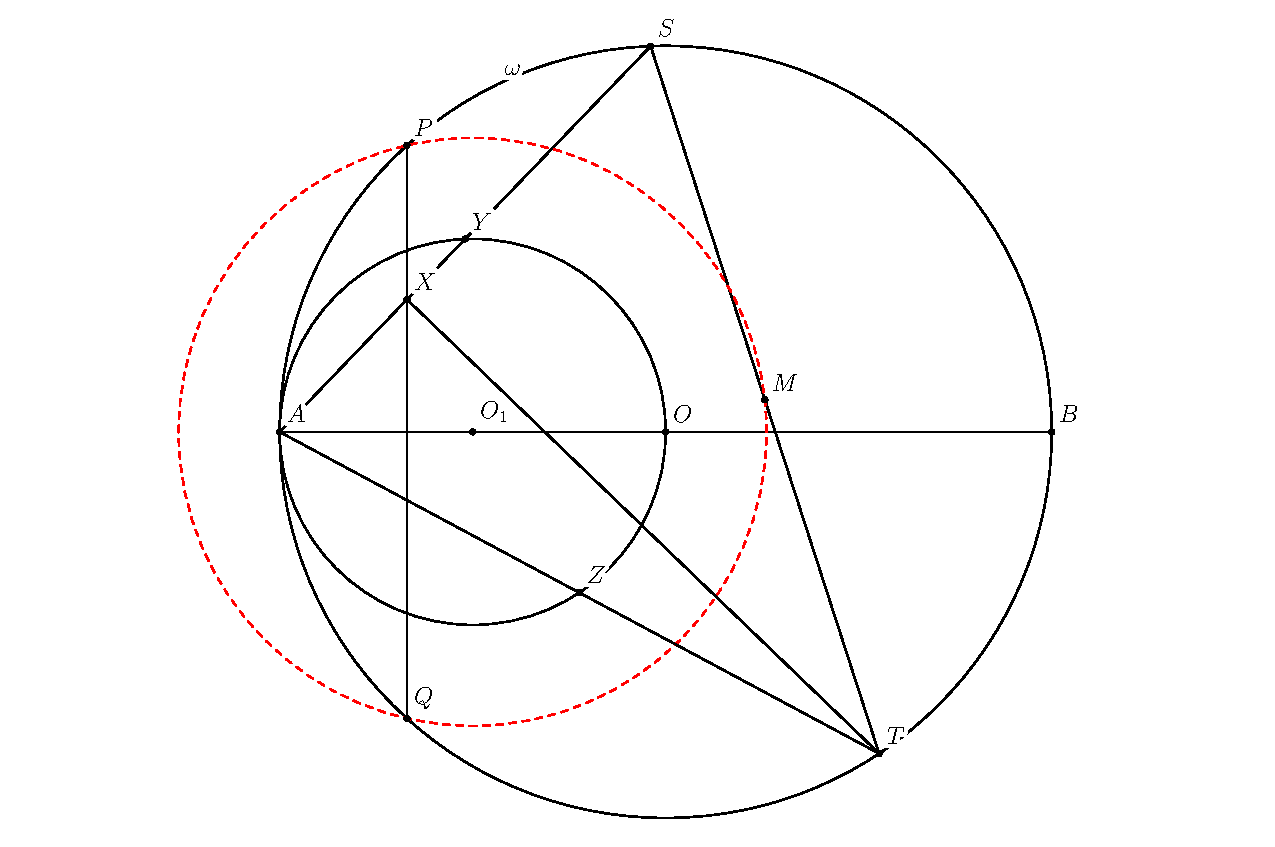
\includegraphics[scale=0.6]{usa2015.pdf}

‎‎
دایره به قطر ‎‎$‎AO‎$‎ ‏را ‎$‎‎‎\omega'‎$‎ در نظر بگیرید. اثبات میکنیم که ‎‎$‎M‎$‎ ‏به روی دایره ای هم مرکز با ‎$‎‎\omega‎'‎$‎ ‏قرار دارد. برای این منظور کافی است اثبات کنیم قوت ‎‎$‎M‎$‎ نسبت به ‎‎$‎\omega'‎$‎ مستقل از ‎‎$‎X‎$‎ ‏است.
\\
بر اساس خطی بودن قوت نقطه میتوانیم بنویسیم:

\begin{align*}
    \mathbf{P}(M,\omega',\omega)&=(\frac12)\mathbf{P}(S,\omega',\omega)+(\frac12)\mathbf{P}(T,\omega',\omega)\\
    \implies Pow_M^{\omega'}&=\frac{AS^2+AT^2-ST^2}{4}\\
    &= \frac{2 AS \dot AT \cos{(\angle A)}}{4}\\
    &=\frac{AP^2}{2}
\end{align*}
پس قوت ‎$M‎$‎‎ ‏نسبت به ‎‎$‎\omega'‎$‎ برابر‎‎ با ثابت ‎‎$‎‎\frac{AP^2}{2}‎$‎‎ ‏که نتیجه میدهد ‎‎$‎M‎$‎ ‏بر روی دایره ای به مرکز وسط ‎‎$‎AO‎$ ‏‎حرکت‎ میکند.

\section{نسبت قوت}

\begin{theo}

\end{theo}

\end{document}